
\chapter{BlooP和FlooP和GlooP}

\section{自我意识和无序}

BlooP、FlooP和GlooP不是神话中的巨人,不是唐老鸭的小侄子们,也不是船沉时发出的冒泡声——它们是三种计算机语言,其中每种都有特殊的用途。这些语言是专门为本书的这一章发明的。它们将被用来解释“递归”这个词的某些新意义——特别是“原始递归”和“一般递归”这两个概念。事实将证明,这些语言有助于阐明TNT中自我相关的机制。

我们似乎很突然地从大脑和心智跳到了数学和计算机科学中的技术。虽然这个跳跃从某些方面来看有点突然,但它还是有意义的。我们已经看到,某种自我意识似乎是意识的关键所在。现在我们要在更形式化的背景下进一步分析“自我意识”,例如在TNT的背景下。在TNT和心智之间还有很大一段距离,但一些想法将会是富有启发性的,或许会以隐喻的方式被传回到我们关于意识的思考之中。

关于TNT的自我意识,令人惊奇的一点就是它密切地联系于自然数中的有序与无序问题。特别是我们将会看到,一个充分复杂以至能反映自身的有序系统不可能是完全有序的——它必定包括某种奇怪的无序特征。对于那些具有某种阿基里斯式想法的读者来说,这将是很难接受的。但是,存在一种“魔术式的”补偿——存在某种关于无序的有序,这本身已经形成了一个研究领域,称为“递归函数论”。遗憾的是,我们所能做到的,只是略微展示一下这个课题的魅力。

\section{可体现性与冰箱}

像“足够复杂”或“足够强有力”及类似的说法,在前面已经多次出现了。但这些说法是什么意思呢?让我们回到龟蟹之战,并问这样一个问题:“是什么使某个东西有资格成为一台唱机的?”螃蟹可能会声称它的冰箱是一台“完备的”唱机。然后为了证明这一点,它可能会随便拿个唱片放在冰箱顶上,说:“你看——它在播放这张唱片了。”而乌龟,如果想要反驳这个禅宗式的行动,就必须说:“不——你的冰箱保真度太低,已经不能算是唱机了:它根本不能重现唱片上记录的声音(更不必说那种让它自我破坏的声音了)”。只有当“唱机X”真是一台唱机时,乌龟才能造出一张叫做“我不能在唱机X上播放”的唱片。乌龟的方法很狡猾,因为它抓的是系统的强项,而非弱项。因此它要求“保真度足够高”的唱机。

对形式化的数论系统来讲也是一样。说TNT是一个形式化的N,其原因是TNT的符号以正确的方式活动:这也就是指它的定理不像冰箱似的一声不响——它们确实说出了N中的真理。当然,"pq"系统中的定理也是这样。"pq"系统也能作为一个“形式化的数论系统”吗?还是说它更像个冰箱?它比冰箱是强一点,但仍然很弱。被"pq"系统所包含的N中的核心真理太少了,因此它还不能称作是一个“数论系统”。

那么,这些N中的“核心真理”是什么呢?它们是“原始递归真理”,这就是说,它们仅仅涉及到“可预测其终止”的计算。这些核心真理在N中的作用就像欧里几得的前四个公设在几何学中的作用一样:它们使你可以在比赛开始前就能淘汰掉某些“力量不够强”的选手。从此以后,“全部原始递归真理的可体现性”将作为我们判别一个系统是否“足够强有力”的标准。

\section{元数学中的岩头之斧}

上述观念的重要性表现在下列关键性的事实之中:如果你有数论的一个足够强有力的形式化体现,那么哥德尔定理就是可应用的,结果你的系统是不完备的。反过来,如果你的系统不足够强有力(即不是所有原始递归真理都是定理),那么因为这个缺陷,它也不完备。这里我们在元数学中碰到了“岩头之斧”的另一种形式化体现:不管系统怎么办,哥德尔之斧总要砍掉它的脑袋!另一点需要注意的是,这完全平行于《对位藏头诗》中的“高低保真度之别”。

实际上,人们发现很弱的系统依然会受到哥德尔方法的攻击。“所有原始递归真理都需要体现成定理”,这个标准过于严格了。这有点像这样一个贼:他只偷“足够阔气”的人,其标准是盗窃对象应当至少带有一百万元现金。幸运的是,对TNT系统来说,我们将能够像这个贼那样动手,因为那里确实有一百万元现金——这就是说,TNT确实包含了所有原始递归真理作为其定理。

现在,在我们进入对原始递归函数的谓词的详细讨论之前,我想把这一章的主题和前几章的主题联系起来,以提供一个更好的背景。

\section{选择适当的过滤器来发现有序}

我们很早就已经看到,形式系统可能是难以驾驭的,因为它们有加长和缩短符号串的规则,这可能会导致在大量符号串中进行无终止的搜索。哥德尔配数法的发现,显示了任何对一个具有特殊的符号性质的串的搜索都有一个算术中的表兄弟:对一个具有相应的特殊算术性质的整数的同构搜索。结果,对于形式系统判定过程的要求,涉及了对整数中不可预测其长度的搜索之谜(一种无序)的解决。在本章前面的对话中,我可能过分强调了和整数有关的问题中显示出的无序现象。事实上,和“妙极性”问题相比,人们已经驯服了一些更复杂的无序现象,发现它们不过是些很温顺的家伙。因此,阿基里斯对数的规则性和可预测性的坚定信仰,应当得到一定的尊敬——特别是由于这反映了到30年代为止几乎所有数学家的信念。为了说明为什么有序与无序的对比是这样一个微妙而有意义的问题,也为了把这一问题和对意义的定位及揭示等问题联系起来,我想引用《量子是实在的吗?》一文中优美而又令人难忘的一段——这是已故的杰·尧奇写的一篇伽利略式的对话:
\begin{quote}
\begin{description}[wide,labelsep=\ccwd,format=\sffamily\itemcolon]
\item[萨尔维亚蒂]假设我给你两个数列,如
\[
7\;8\;5\;3\;9\;8\;1\;6\;3\;3\;9\;7\;4\;4\;8\;3\;0\;9\;
6\;1\;5\;6\;6\;0\; 8\;4\;\dotsc
\]
和
\[
1,\;-\frac13,\;+\frac15,\;-\frac17,\;+\frac19,\;
-\frac1{11},\;+\frac1{13},\;-\frac1{15},\;\dotsc
\]
如果我问你,辛普利奇奥,第一个序列的下一个数是什么,你会怎样说?

\item[辛普利奇奥]我无法告诉你。我觉得它是个随机序列,其中没有规律。

\item[萨尔维亚蒂]那么第二个序列呢?

\item[辛普利奇奥]这个容易,下一个一定是$+1/17$。

\item[萨尔维亚蒂]正确。但如果我告诉你第一个序列也是按某个规律构造的,而且这个规律事实上和你刚才在第二个序列中发现的一样,你会说什么?

\item[辛普利奇奥]我看这不大可能。

\item[萨尔维亚蒂]但事实的确如此。因为第一个序列只不过是第二个序列的和的十进制小数部分(展开式)的开始几位。这个和是$\uppi/4$。

\item[辛普利奇奥]你用的数学技巧太多,但我看不出这与抽象和实在有什么关系。

\item[萨尔维亚蒂]和抽象的关系显而易见。除非你已经通过抽象过程开发了一种过滤器,用它可以看出在表面的随机性背后的简单结构,否则第一个序列看上去就是随机的。

自然规律恰恰是以这种方式被发现的。自然只是提供给我们大量的现象,它们表面上杂乱无章,直到我们选择了某些有意义的事件,而且把它们从特定的,关系不大的环境中抽象出来,使它们成为理想化的时候为止。只有那时它们才会展现出光彩夺目的真实结构。

\item[萨哲杜]这个想法太妙了!由此看来当我们设法理解自然时,我们应当把现象看作待理解的消息。只不过每个消息在我们为它设立一种编码之前好像是随机的。这种编码表现为一种抽象,就是说,我们有选择地把某些无关的东西忽略掉,这样就通过一种自由选择选取了消息的部分内容。这些无关信号构成了“背景噪声”,它们将限制我们的消息的精确性。

    但由于这种编码不是绝对的,在同一组作为原材料的数据中就可能存在着多个消息,因此改变编码就会在某些以前认为只是噪声的东西中发现同样深刻的意义。相反地,在新的编码中以前的消息可能会变得没有意义。

    这样一种编码就预先设定了在不同的、互补的方面之间的一种自由选择。每个方面都同样自称是“真实的”,如果我可以用这个可疑的词的话。

    在这些方面之中,有些可能目前还完全不为我们所知,但它们可能把自己暴露给一个具有完全不同的抽象系统的观察者。

    但请告诉我,萨尔维亚蒂,这样,我们怎么能仍然声称我们在客观的实在世界中发现了某些事物呢?这难道不是意味着我们只不过是根据自己的想象在构造事物,而实在仅仅存在于我们自身之中吗?

\item[萨尔维亚蒂]我不认为一定是这样的,但这是一个需要进一步反思的问题。\note{尧奇,《量子是实在的吗?》,第63--65页。}
\end{description}
\end{quote}

在这里,尧奇所涉及到的消息不是来自一个“有感知能力的物体”,而是来自自然界本身。我们在第六章提出的关于意义和消息的关系的问题同样适用于来自自然的消息。自然是无序的还是模式化的?智能在确定这个问题的答案的过程中能起什么作用?

从哲学中退出来,我们仍能考虑表面上的随机序列中深藏的规律性。第五章中的函数$\mQ(n)$是否也具有一个简单的非递归解释?是不是每个问题都像《一首无的奉献》中提到的那片果树林一样,从某个特定的角度看进去,其中的秘密就一览无余了?还是说在数论中存在着一些不论从哪个角度看都是神秘的问题?

有了这段开场白,我觉得现在应该继续前进,去定义所谓“长度可预测的搜索”的精确意义了。这将用BlooP语言来完成。

\section{BlooP语言的基本步骤}

我们的议题是搜寻具有各种性质的自然数。为了讨论任意搜索的“长度”,我们必须定义一些基本“步骤”,任何搜索都由它们组成。这样,搜索长度就可以根据其中的步骤数来度量。被我们当作基本步骤的有:
\begin{itemize}
\item 两个自然数相加;
\item 两个自然数相乘;
\item 确定两个数是否相等;
\item 确定两个数的相对大小。
\end{itemize}

\section{循环和上界}

如果我们想用这些步骤严格地构造一个测试,例如测试一个数是否是素数,我们很快就会发现必须在其中包含一个“控制结构”——即对操作次序的描述:何时需要回过头来重新尝试某些东西,何时跳过一些步骤,何时停止,以及诸如此类的事情。

在典型的情况下,任何“算法”——即对任务完成过程的明确描述——都由下列成分组成:\pnum{1}需完成的特定运算,\pnum{2}控制语句。因此,当我们为表示长度可预测的计算开发我们的语言时,我们必须同时包括基本控制结构。事实上,BlooP的特色也恰在于其有限的控制结构集。它不允许你转移到任意的步骤或无限制地循环某一步骤。在BlooP中,基本上唯一的控制结构就是“有界循环”(即“bounded loop”,这也正是“BlooP”的来历):重复执行一组指令,重复次数不能大于某个预先确定的最大值。这个最大值称为该循环的“上界”,或“顶”。如果顶是$300$,那么这个循环可以进行$0$次、$7$次或$300$次——但不能是$301$次。

在一个程序中,并不要求程序员准确地给出所有上界的数值——事实上它们是无法预知的。但是,每个上界都可以在进入该循环之前通过计算来确定。例如,如果你要计算$2^{3^n}$的值,就该设置两个循环。首先,你求出$3^n$的值,这包括$n$次乘法。然后,你求$2$的$3^n$次方,这包括$3^n$次乘法。这样,第二个循环的上界是第一个循环的计算结果。

下面说明你怎样才能把这个过程表示在一个BlooP程序之中:

\newcommand*\CM{\>\small}
\newcommand*\PROCEDURE[2]{\inst{DEFINE PROCEDURE ``#1''} $[#2]$:}
\newcommand*\BEGINBLOCK[1]{\inst{BLOCK} $#1$: \inst{BEGIN}}
\newcommand*\ENDBLOCK[1]{\inst{BLOCK} $#1$: \inst{END}}
\newcommand*\LOOP[1]{\inst{LOOP} $#1$ \inst{TIMES}:}
\newcommand*\LOOPATMOST[1]
  {\inst{LOOP} \inst{AT} \inst{MOST} $#1$ \inst{TIMES}:}
\newcommand*\ABORTLOOP[1]{\inst{ABORT} \inst{LOOP} $#1$;}
\newcommand*\IFTHEN[1]{\inst{IF} $#1$, \inst{THEN}:}
\newcommand*\QUITBLOCK[1]{\inst{QUIT} \inst{BLOCK} $#1$;}

\begin{tabbing}
\indent \= \qquad \= \tabindent{0em} \= \kill
\PROCEDURE{TWO-TO-THE-THREE-TO-THE}{N} \\
 \> \>                                    \CM 定义过程名和参数$N$\\
\BEGINBLOCK{0} \> \>                      \CM 第$0$块开始 \+\\
  $\CELL(0)\impliedby 1$; \>              \CM 把“$1$”送入$0$号单元\\
  \LOOP{N} \>                             \CM 循环执行$N$次\\
  \BEGINBLOCK{1} \>                       \CM 第$1$块开始\+\\
    $\CELL(0)\impliedby 3\times\CELL(0)$; \CM $0$号单元内容乘“$3$”结果\\
                                          \CM 仍送入$0$号单元 \-\\
  \ENDBLOCK{1} \>                         \CM 第$1$块结束 \\
  $\CELL(1)\impliedby 1$; \>              \CM 把“$1$”送入$1$号单元 \\
  \LOOP{\CELL(0)} \>                      \CM 循环次数在$0$号单元中 \\
  \BEGINBLOCK{2} \>                       \CM 第$2$块开始 \+\\
    $\CELL(1)\impliedby 2\times\CELL(1)$; \CM $1$号单元内容乘“$2$”结果\\
                                          \CM 仍送入$1$号单元 \-\\
  \ENDBLOCK{2} \>                         \CM 第$2$块结束 \\
  \inst{OUTPUT} $\impliedby \CELL(1)$;\>  \CM $1$号单元内容送入输出单元  \-\\
\ENDBLOCK{0} \> \>                        \CM 第$0$块结束
\end{tabbing}

\section{BlooP的约定}

能够看着一个用计算机语言书写的算法,指出它是做什么的,这需要学习。但是,我希望这个算法足够简单,不必仔细研究就能理解。在上述程序中,定义了一个“过程”,它带有一个“输入参数”$N$,它的“输出”就是所要得到的值。

这个过程定义采用所谓“块结构”,这就是说其中某些部分可以被看作一个单元,或“块”。在一块中的所有语句可以被当作一个单元来执行。每一块都有个编号(最外面一层是\inst{BLOCK} $0$),而且用\inst{BEGIN}和\inst{END}标记开始和结束。在我们这个例子中,\inst{BLOCK} $1$和\inst{BLOCK} $2$每个仅含一个语句——但不久你就会见到更长的块。一个\inst{LOOP}语句总是意味着重复地执行紧随其后的块。正像在上例中所见到的,块可以互相嵌套。

上述算法的策略前面已经描述过了。你首先取一个辅助变量,叫$\CELL(0)$,把它的初值赋为$1$,然后,在一个循环中反复地把其值乘以$3$,直到这样做完$N$次为止。下一步,你对$\CELL(1)$做类似处理——把它置成$1$,反复乘$2$,做$\CELL(0)$次,然后停止。最后,你把$\CELL(1)$中的值赋给\inst{OUTPUT}。这个值就是要传回给外部世界的——这是该过程唯一的外部可见行为。

关于所用的记号,在这里还有几点需要说明。首先,左箭头“$\impliedby$”的意思是这样:

\begin{block}
求出其右边公式的值,然后把结果赋给其左边的\inst{CELL}(或\inst{OUTPUT})。
\end{block}
因此$\CELL(1)\impliedby 3\times\CELL(1)$这条命令的意义就是把存在$\CELL(1)$中的值乘$3$倍。你可以把每个$\CELL$想象成某个计算机的存贮器中的一个字。在一个$\CELL$和一个真实的字之间的唯一区别就是:后者只能存放某个确定限度之内的整数,而我们允许一个$\CELL$存放任意自然数,不管有多大。

在BlooP中,每个过程在被调用时都能得出一个值——即称为\inst{OUTPUT}的变量的值。在开始执行任何过程时,\inst{OUTPUT}都把$0$值作为其缺席选择值。这样,即使过程根本没给\inst{OUTPUT}重新赋值,\inst{OUTPUT}也能始终有一个明确定义的值。

\section{IF条件语句和分支}

现在让我们看另一个过程,它将展示BlooP的其它特点,这些特点使该语言更加具有一般性。如果只会做加法,你怎样才能求出$M-N$的值呢?窍门在于把各种各样的数和$N$相加,直至你发现一个与$N$的和等于$M$的数为止。但是如果$M$小于$N$会发生什么情况呢?如果我们想从$2$中取走$5$会怎样?这在自然数域中是没有答案的。但我们希望我们的BlooP过程不管怎样应当给出一个答案——比如说$0$。下面就是一个做减法的BlooP过程:

\begin{tabbing}
\indent \= \qquad \= \tabindent{-1em} \= \kill
\PROCEDURE{MINUS}{M,N} \> \>    \CM 定义过程名和变量$M$ \\
\BEGINBLOCK{0} \> \>            \CM 第$0$块开始 \+\\
  \IFTHEN{M<N} \>               \CM 若$M<N$,则:\\
  \QUITBLOCK{0} \>              \CM 退出第$0$块\\
  \LOOPATMOST{M+1} \>           \CM 循环至多$M+1$次;\\
  \BEGINBLOCK{1} \>             \CM 第$1$块开始 \+\\
    \IFTHEN{\inst{OUTPUT}+N=M}  \CM 若$\inst{OUTPUT}+N=M$,则:\\
    \ABORTLOOP{1}               \CM 中止循环$1$\\
    $\inst{OUTPUT}\impliedby\inst{OUTPUT}+1$;
                                \CM \inst{OUTPUT}的值加$1$,送回 \-\\
  \ENDBLOCK{1} \>               \CM 第$1$块结束\-\\
\ENDBLOCK{0} \> \>              \CM 第$0$块结束
\end{tabbing}

这里我们利用了\inst{OUTPUT}开始时为$0$这一隐含性质。如果$M$小于$N$,那么减法就是不可能的,我们只需直接跳到\inst{BLOCK} $0$的末尾,同时答案是$0$。这就是\inst{QUIT} \inst{BLOCK} $0$这一行的意思。但如果$M$不小于$N$,那么我们就越过这条\inst{QUIT}语句,按顺序执行下一条命令(在这里是个\inst{LOOP}语句)。这就是\inst{IF}语句在BlooP中的工作方式。

这样,我们就进入了\inst{LOOP} $1$。这样称呼它,是因为它要重复执行的块是\inst{BLOCK} $1$。我们试着把$0$加到$N$上,然后是$1$、$2$、$3$……直到我们找到那个能导出$M$的数。这时我们对当前循环做\inst{ABORT},即跳到紧跟着标识循环块底的\inst{END}后面的一条语句。在上述例子中,我们跳到了\inst{BLOCK} $1$: \inst{END}的后面,即到达了算法的最后一条语句,而且任务已经完成了。现在\inst{OUTPUT}中放的就是正确答案。

注意,往下跳有两种不同的指令:\inst{QUIT}和\inst{ABORT}。前者从属于块,后者从属于循环。\inst{QUIT} \inst{BLOCK} $n$意味着跳到\inst{BLOCK} $n$的最后一行,而\inst{ABORT} \inst{LOOP} $n$意味着跳到\inst{BLOCK} $n$的最后一行之后。只有在一种情况下二者的区别是重要的:当你在一个循环之中,想要继续循环,但又要退出这一轮所在的块。这时你用\inst{QUIT}就能达到预期的效果。

还应当注意的是在循环上界前面注有\inst{AT} \inst{MOST}(至多),这告诫你循环可能在达到上界之前就被中止了。

\section{自动组块}

下面是BlooP的最后两个需要加以说明的特点,它们都是非常重要的。其一是:一旦一个过程已经被“定义”了,它就可以在后面的过程定义中被“调用”。其效果是一旦某个操作在一个过程中被定义了,它就会被认为和基本步骤一样简单。这样,BlooP就具有了自动组块的特点。你可以把这和一个溜冰好手学习新花样的过程相比:他不是把新动作看作长长的基本肌肉活动序列,而是看作以前学过的一些动作的组合,而那些动作自身又是用更早所学的动作所组成的,如此等等——这种嵌套或组块可以上溯许多层次,直至遇到基本肌肉活动为止。这样,BlooP程序的能力就和溜冰者的技能一样,可以突飞猛进地增长了。

\section{BlooP测试}

BlooP的另一个特点是:某些特定过程可以用\inst{YES}或\inst{NO}作为其输出,而不是输出一个整数的值。这种过程是“测试”,而非“函数”。为了说明这个区别,测试的名字必须以一个问号结束。另外,在一个测试中,\inst{OUTPUT}的缺省值当然不能是$0$,而是\inst{NO}。

让我们看一个例子,其中把BlooP的最后这两个特点表现在一个算法里。这个算法要测试一个函数的自变量是否是素数。

\begin{tabbing}
\indent \= \qquad \= \tabindent{0em} \= \kill
\PROCEDURE{PRIME}{N} \> \>                     \CM 定义过程名和变量$N$ \\
\BEGINBLOCK{0} \> \>                           \CM 第$0$块开始\+\\
  \IFTHEN{N=0} \>                              \CM 若$N=0$,则:\\
  \QUITBLOCK{0} \>                             \CM 退出第$0$块\\
  $\CELL(0)\impliedby 2$; \>                   \CM 把$\CELL(0)$置成$2$\\
  \LOOPATMOST{\inst{MINUS}[N,2]} \\
  \>                                           \CM 循环至多$N-2$次\\
  \BEGINBLOCK{1} \>                            \CM 第$1$块开始\+\\
    \IFTHEN{\inst{REMAINDER}[N,\CELL(0)]=0} \\
                                               \CM 若$N$除以$\CELL(0)$余$0$,则:\\
    \QUITBLOCK{0}                              \CM 退出第$0$块\\
    $\CELL(0) \impliedby \CELL(0)+1$;          \CM $\CELL(0)$的值加$1$\-\\
  \ENDBLOCK{1} \>                              \CM 第$1$块结束\\
  $\inst{OUTPUT} \impliedby \inst{YES}$;\>     \CM 把\inst{OUTPUT}置成\inst{YES}\-\\
\ENDBLOCK{0} \> \>                             \CM 第$0$块结束
\end{tabbing}

注意,我在这个算法中调用了两个过程:\inst{MINUS}和\inst{REMAINDER}(假设后者已经事先定义了,你可以自己完成这个定义,\inst{REMAINDER}$[N,R]$的作用是求$N$除以$R$所得的余数)。这个素数测试过程的工作方式是逐个检查$N$可能有的因子,从$2$开始直到$N-1$为止。如果其中某一个能整除$N$(即余数为$0$),则跳到过程尾部,由于此时\inst{OUTPUT}仍然保有其缺省值,故答案为\inst{NO}。仅当$N$没有整数因子时,它才能通过整个\inst{LOOP} $1$,那时我们会遇到语句$\inst{OUTPUT}\impliedby\inst{YES}$,执行了这个语句后,过程就结束了。

\section{BlooP程序包含了过程组成的链}

我们已经看到了在BlooP中怎样定义过程,但过程定义只是一个程序的一部分。一个“程序”包括一条“过程定义链”(其中每个过程仅仅调用前面定义的过程),还可能跟着一个或多个对所定义过程的“调用”。例如,过程\inst{TWO-TO-THE-THREE-TO-THE}的定义和后面跟着的调用
\[
\text{\inst{TWO-TO-THE-THREE-TO-THE}}[2]
\]
合起来构成了一个完整的BlooP程序,它的运行结果是$512$。

如果你只有一条过程定义链,那什么东西都不会被执行。它们就在那里等着调用,等着用特定的数值启动它们。这就像一台绞肉机等着肉来绞——或者说更像一串连在一起的绞肉机,前面一台绞完了就送进后一台……对于绞肉机来说,这种安排可能没什么必要,但对于BlooP程序来说,这种结构是非常重要的。我们可以可以称它为一个“待调用程序”。这个概念显示在\fig{72}中。

\begin{lrbox}{\TEMPBOX}%
\begin{tikzpicture}[trim right=(OPU)]
\path[every node/.style={draw,dashed,rounded corners=2mm,
        font=\linespread{1}\selectfont,align=center,
        inner xsep=3mm,inner ysep=2mm}]
  node [name=A]                   { 过程定义 \\ $\#1$ }
  node [name=B,below =  3mm of A] { 过程定义 \\ $\#2$ }
  node [name=C,below =  3mm of B] { 过程定义 \\ $\#3$ }
  node [name=D,below = 10mm of C] { 过程定义 \\ $\#k$ };
\path ($(C)!.5!(D)$) node[rotate=90] {\ldots\ldots};
\draw[<<<.-.<<<] (D.west) ++(2mm,3mm)   coordinate (IP)
  -- +(-18mm,0) node[at end,above,anchor=south west]{输入};
\draw[>>>.-.>>>] (D.east) ++(-2mm,-3mm) coordinate (OP)
  -- +(18mm,0)  node[at end,above,anchor=south east]{输出};
\path (IP) ++(-6mm,1mm) coordinate (IPU)
      (IP) ++(-6mm,-1mm) coordinate (IPD)
      (OP) ++(6mm,1mm) coordinate (OPU)
      (OP) ++(6mm,-1mm) coordinate (OPD);
\draw (IPU) |- ([yshift= 3mm]A.north) -| (OPU)
      (IPD) |- ([yshift=-3mm]D.south) -| (OPD);
\end{tikzpicture}
\end{lrbox}

\begin{figure}
%\includegraphics[height=.9\textheight]{img_072.png}
\thisfloatsetup{capbesidesep=qquad,capbesideposition={right,center}}
\fcapside[\FBwidth]{\usebox\TEMPBOX}{\caption[一个待调用的BlooP程序的结构。]
  {一个待调用的BlooP程序的结构。由于这个程序是自足的,每个过程定义中只能调用定义在它前面的过程。}}
\end{figure}

现在BlooP是我们用来定义可预知终止的计算的语言。可以用BlooP来计算的函数的标准名称是“原始递归函数”;而可以用BlooP测试来验证的性质的标准名称是“原始递归谓词”。这样函数$2^{3^n}$就是个原始递归函数,而命题“$n$是个素数”则是个原始递归谓词。

凭直觉就能看出哥德巴赫性质是原始递归的。为了使其明确化,这里有一个用BlooP写的过程定义,来显示如何测试这一性质是否存在:

\begin{tabbing}
\indent \= \qquad \= \qquad \= \tabindent{0em} \= \kill
\PROCEDURE{GOLDBACH}{N} \>\>\>   \CM 定义过程名和变量$N$\\
\BEGINBLOCK{0} \> \> \>                    \CM 第$0$块开始\+\\
  $\CELL(0)\impliedby 2$; \> \>            \CM 把$\CELL(0)$置成$2$\\
  \LOOPATMOST{N} \> \>                     \CM 循环至多$N$次\\
  \BEGINBLOCK{1} \> \>                     \CM 第$1$块开始\+\\
\pushtabs
    \inst{IF} \= $\{$ \= $\inst{PRIME?}[\CELL(0)]$ \=\\
      \> \> $\inst{AND}\;\inst{RPIME?}[\inst{MINUS}[N,\CELL(0)]]\}$,\\
      \> \> \quad\inst{THEN}; \`\small 若$\CELL(0)$和$N-\CELL(0)$均为素数,则:\\
\poptabs
    \BEGINBLOCK{2} \> \CM 第$2$块开始\+\\
      $\inst{OUTPUT}\impliedby\inst{YES}$; \CM 把\inst{OUTPUT}置成\inst{YES}\\
      \QUITBLOCK{0}                        \CM 退出第$0$块\-\\
    \ENDBLOCK{2} \>                        \CM 第$2$块结束\\
    $\CELL(0)\impliedby\CELL(0)+1$; \>     \CM $\CELL(0)$加$1$\-\\
  \ENDBLOCK{1} \> \>                       \CM 第$1$块结束\-\\
\ENDBLOCK{0} \> \> \>                      \CM 第$0$块结束
\end{tabbing}
和通常一样,我们先假设\inst{NO},直到证明\inst{YES}为止。而且我们是靠一股蛮劲在其和为$N$的数对之中进行搜索。如果两个数均为素数,我们就退出最外层的块,否则我们就返回去再试,直至穷尽全部可能性为止。

(警告:哥德巴赫性质是原始递归的,但这一事实并没有使“是否所有的数都具有哥德巴赫性质?”成为一个简单的问题——远非如此!)

\section{推荐的练习题}

你能写一个类似的过程来测试乌龟性质(或阿基里斯性质)是否存在吗?如果能,就请写出来。如果不能,是仅仅因为你不知道上界,还是因为在BlooP中刻画这样的算法时遇到了根本性的障碍?如果对在对话中提出的“妙极性”性质提同样的问题,会得出什么答案?

下面我将列出一些函数和性质,你最好花一些时间来确定你是否相信它们是原始递归的(即可用BlooP编程序)。这意味着你必须认真考虑它们所要求的计算中包含哪些操作,以及是否能给出其中涉及的全部循环的项。

\begin{itemize}[labelindent=0pt]
\item $\inst{FACTORIAL}[N]=N!$($N$的阶乘)。例如:
\begin{itemize}
  \item $\inst{FACTORIAL}[4]=24$
\end{itemize}

\item $\inst{REMAINDER}[M,N]=\text{用$N$除$M$所得的余数}$。例如:
\begin{itemize}
  \item $\inst{REMAINDER}[24,7]=3$
\end{itemize}

\item $\inst{PI-DIGIT}[N]=\text{$\uppi$在小数点后的第$N$位数字}$。例如:
\begin{itemize}
  \item $\inst{PI-DIGIT}[1]=1$
  \item $\inst{PI-DIGIT}[2]=4$
  \item $\inst{PI-DIGIT}[1000000]=1$
\end{itemize}

\item $\inst{FIBO}[N]=\text{斐波那契数列的第$N$项}$。例如:
\begin{itemize}
  \item $\inst{FIBO}[9]=34$
\end{itemize}

\item $\inst{PRIME-BEYOND}[N]=\text{大于$N$的最小素数}$。例如:
\begin{itemize}
  \item $\inst{PRIME-BEYOND}[33]=37$
\end{itemize}

\item $\inst{PERFECT[N]}=\text{第$N$个“完全”数}$(一个数的所有约数之和等于它本身,如$28=1+2+4+7+14$),例如:
\begin{itemize}
  \item $\inst{PERFECT[2]}=28$
\end{itemize}

\item $\inst{PRIME?}[N]=\inst{YES}$若$N$是素数,否则为\inst{NO}。

\item $\inst{PERFECT?}[N]=\inst{YES}$若$N$是完全数,否则为\inst{NO}。

\item $\inst{TRIVIAL?}[A,B,C,N]=\inst{YES}$若$A^N+B^N=C^n$成立,否则为\inst{NO}。例如:
\begin{itemize}
  \item $\inst{TRIVIAL?}[3,4,5,2]=\inst{YES}$
  \item $\inst{TRIVIAL?}[3,4,5,3]=\inst{NO}$
\end{itemize}

\item $\inst{PIERRE?}[A,B,C]=\inst{YES}$若$A^N+B^N=C^N$可以被某个大于$1$的$N$值所满足,否则为\inst{NO}。例如:
\begin{itemize}
  \item $\inst{PIERRE?}[3,4,5]=\inst{YES}$
  \item $\inst{PIERRE?}[1,2,3]=\inst{NO}$
\end{itemize}

\item $\inst{FERMAT?}[N]=\inst{YES}$若$A^N+B^N=C^N$可以被某一组正数$A$、$B$、$C$所满足,否则为\inst{NO}。例如:
\begin{itemize}
  \item $\inst{FERMAT?}[2]=\inst{YES}$
\end{itemize}

\item $\inst{TORTOISE-PAIR?}[M,N]=\inst{YES}$若$M$和$M+N$均为素数,否则为\inst{NO}。例如:
\begin{itemize}
  \item $\inst{TORTOISE-PAIR?}[5,1742]=\inst{YES}$
  \item $\inst{TORTOISE-PAIR?}[5,100]=\inst{NO}$
\end{itemize}

\item $\inst{TORTOISE?}[N]=\inst{YES}$若$N$为两个素数之差,否则为\inst{NO}。例如:

\begin{itemize}
  \item $\inst{TORTOISE?}[1742]=\inst{YES}$

  \item $\inst{TORTOISE?}[7]=\inst{NO}$
\end{itemize}

\item $\inst{WJU-WELL-FORMED?}[N]=\inst{YES}$若$N$可以看作"WJU"系统中的一个良构串,否则为\inst{NO}。例如:

\begin{itemize}
  \item $\inst{WJU-WELL-FORMED?}[310]=\inst{YES}$

  \item $\inst{WJU-WELL-FORMED?}[415]=\inst{NO}$
\end{itemize}

\item $\inst{WJU-PROOF-PAIR?}[M,N]=\inst{YES}$若在"WJU"系统中可以把串序列$M$看作串$N$的一个推导,否则为\inst{NO}。例如:
\begin{itemize}
  \item $\inst{WJU-PROOF-PAIR?}[3131131111301,301]=\inst{YES}$
  \item $\inst{WJU-PROOF-PAIR?}[311130,30]=\inst{NO}$
\end{itemize}

\item $\inst{WJU-THEOREM?}[N]=\inst{YES}$若$N$对应的"WJU"系统中的串是一个定理,否则为\inst{NO}。例如:
\begin{itemize}
  \item $\inst{WJU-THEOREM?}[311]=\inst{YES}$
  \item $\inst{WJU-THEOREM?}[30]=\inst{NO}$
  \item $\inst{WJU-THEOREM?}[701]=\inst{NO}$
\end{itemize}

\item $\inst{TNT-THEOREM?}[N]=\inst{YES}$若$N$对应的TNT串是个定理,例如:
\begin{itemize}
  \item $\inst{TNT-THEOREM?}[666111666]=\inst{YES}$
  \item $\inst{TNT-THEOREM?}[223666111666]=\inst{NO}$
  \item $\inst{TNT-THEOREM?}[7014]=\inst{NO}$
\end{itemize}

\item $\inst{FALSE?}[N]=\inst{YES}$若$N$对应的TNT串是数论中的一个假命题,否则为\inst{NO}。例如:
\begin{itemize}
  \item $\inst{FALSE?}[666111666]=\inst{NO}$
  \item $\inst{FALSE?}[223666111666]=\inst{YES}$
  \item $\inst{FALSE?}[7014]=\inst{NO}$
\end{itemize}

\end{itemize}

后面七个题目与我们将要进行的元数学探索关系密切,因此很值得你认真分析。

\section{可表示性和可体现性}

在继续讨论一些关于BlooP及其“亲戚”FlooP的问题之前,让我们先回顾一下当初引进BlooP的原因,并把它和TNT联系起来。我在前面说过,一旦全部原始递归的概念对一个形式系统来说都是可体现的,那么这个系统就达到了使用哥德尔方法所需的“临界质量”。这到底意味着什么呢?首先,我们必须区别这样两个概念:可表示性和可体现性。“表示”一个谓词只是从自然语言到严格的形式化表述的翻译问题。这和该谓词是不是定理没有关系。而“体现”一个谓词就是强得多的概念了。这意味着:
\begin{enumerate}
\item 该谓词的全部为真的例均为定理;
\item 全部为假的例均为非定理。
\end{enumerate}

“例”在这里是指用数值取代谓词中所有自由变量后所得到的串。例如,谓词$m+n=k$在"pq"系统中是可体现的,因为该谓词的每个为真的例都是定理,每个为假的例都是非定理。这样,任何具体的加法算式,无论真假,都能被译成"pq"系统中的“可判定串”。但是,"pq"系统不能表示——更不要说体现——自然数的任何别的性质。因此在对数论进行形式化的竞争之中,它的确不是一个强有力的候选。

而TNT的优点是能够表示数论中的任何谓词。例如,很容易写一个TNT串来表示谓词“$b$具有乌龟性质”。因此,根据表示能力来看,TNT满足我们的全部要求。

但是,问“在TNT中哪些性质是可体现的?”,这恰恰就是问“TNT作为一个公理系统有多强?”。是不是所有可能的性质在TNT中都是可体现的?若是如此,那么TNT就能回答数论中的任何问题,它就是完全的。

\section{原始递归谓词在TNT中是可体现的}

虽然完全性将被发现是个幻梦,TNT至少相对于原始递归谓词来说还是完全的。换句话说,如果数论中的某个陈述的真假能用计算机在一个长度可预知的时间段中判定,那它在TNT中一定也是可判定的。也可以把这个问题表述成如下形式

\begin{block}
如果能为自然数的某个性质写出一个BlooP测试,那么这个性质在TNT中是可体现的。
\end{block}

\section{存在非原始递归的函数吗?}

用BlooP测试可以检查许多种不同的性质,包括一个数是否为素数或完全数、是否具有哥德巴赫性质、是否是$2$的幂,如此等等。这自然地会使人考虑是不是数的每种性质都能被某个适当的BlooP程序所检查。虽然我们现在还无法测试一个数是否是妙极的,但我们不必过于因此心烦意乱,因为这也许仅仅是由于我们对妙极性还缺乏认识,随着进一步的挖掘,我们也许会为其中包含的循环上界发现一个通用的公式。那时就可以马上为妙极性写出一个BlooP测试了。对乌龟性质可能也是同样的。

因此,这个问题实质上是“是否总能给出运算长度的上界——还是说在自然数系统中存在一种内在的混乱,致使有时无法事先预测运算的长度?”令人震惊的是,恰好是后一种情况出现了,其原因我们不久就会看到。这种事情准会把毕达哥拉斯——他第一个证明了二的平方根是无理数——气昏了头。在我们的论证中,将使用享有盛名的“对角线法”,这是由集合论的奠基人康托尔发现的。

\section{B库、索引编号和蓝程序}

让我们首先设想一个新奇的概念:装着所有可能的BlooP程序的库。不用说,这个库——“B库”是个无穷大的库。我们要考虑由B库通过三个连续的过滤操作所得到的一个子库。第一个过滤器为我们选出其中的“待调用”程序。然后我们再去掉这个子库中的全部“测试”,只留下“函数”(顺便说明一下,在待调用程序中,链中的最后一个过程决定了整个程序应当被看成是测试还是函数)。第三个过滤器将选出那些恰有一个输入参数的函数(同样只是指链中最后一个过程)。剩下来的是一个包含所有这样的待调用BlooP程序的完整库:这些程序计算那些恰有一个输入参数的函数。

让我们称这些特殊的BlooP程序为“蓝程序”(Bloo的发音在英语里和“蓝”[blue]的发音很相近,而P是“程序”[program]的首字母)。现在我们要做的事是为每个蓝程序指定一个互不混淆的“索引编号”。怎样做呢?最简单的办法——我们正是要这样做——就是根据长度把它们排列起来:可能的蓝程序中最短的为$1$号,次短的为$2$号,等等。当然,会有许多长度相同的程序。为解决这个问题,我们使用字典次序。在这里,“字典次序”是在拓广的意义下使用的,其中字母表里包括BlooP中的所有附加字符,以某一次序排列起来,例如下面这样:
\[
\begin{array}{*{14}{c}}
A&B&C&D&E&F&G&H&I&J&K&L&M&N \\
O&P&Q&R&S&T&U&V&W&X&Y&Z&+&\times \\
0&1&2&3&4&5&6&7&8&9&\Leftarrow&=&<&> \\
(&)&[&]&\{&\}&-&'&?&:&;&,&.&
\end{array}
\]
——注意:其中最后一个是个空格!这样,一共有五十六个字符。为方便起见,我们可以把所有长度为$1$的蓝程序放在第一列,两个字符组成的程序放在第$2$列,等等。显然前几列完全是空的,而后面一些列中有许多许多项(虽然每一列中的项数是有限的)。排在第一的蓝程序大概是这样一个:

\begin{center}
\begin{tabular}{ll}
\PROCEDURE{A}{B} & 定义过程名和参数$B$\\
\BEGINBLOCK{0}   & 第$0$块开始\\
\ENDBLOCK{0}     & 第$0$块结束
\end{tabular}
\end{center}
这个程序实在有点傻:不管输入是什么,输出值总是$0$。它出现在第$56$列中,因为它有$56$个字符(请数一下必要的空格,包括那些隔开相邻两行的空格)。

在遇到第$56$列之后不久,后面的列变得越来越满,因为把符号组合起来形成蓝程序的方法实在太多了。不过不要紧——我们不想设法把这个无穷无尽的目录表列出来。抽象地说,我们所关心的是,这个目录表应当是良定义的,即每个蓝程序能从中得到一个唯一确定的索引编号。这才是关键所在。

让我们这样指示被第$k$个蓝程序所计算的函数:
\[
\text{蓝程序}\{\#k\}[N]
\]
在这里,$k$是该程序的索引编号,$N$是唯一的输入参数。例如,蓝程序$\#12$可以是送回其输入值的二倍的那个函数:
\[
\text{蓝程序}\{\#12\}[N]=2\times N
\]
上述等式的意义是:左面指定的程序将给出一个返回值,这个值和人从右面的常规代数公式中算出的相等。作为另一个例子,或许第$5000$个蓝程序计算其输入参数的立方:
\[
\text{蓝程序}\{\#5000\}[N]=N^3
\]

\section{对角线法}

好,现在我们就要耍那个“花招”了,即使用康托尔的对角线法。我们将用这个蓝程序的目录表定义一个单变量函数——“蓝对角”$[N]$——而且将会发现这个函数根本不在表中(这就是把它的名字加上引号的原因)。而“蓝对角”很显然是个良定义的单变量可计算函数,这样我们就不得不下结论说,存在一些不能在BlooP中编程序的函数。

下面就是“蓝对角”$[N]$的定义:
\begin{equation}\label{eq:blue1}
\text{“蓝对角”}[N]=1+\text{蓝程序}\{\#N\}[N]
\end{equation}
我们的策略是:把每台“绞肉机”的索引编号送给它自己去加工,然后把它的输出值加$1$。为了说清楚这一点,让我们找出“蓝对角”$[12]$。我们已经看到蓝程序\null$\{\#12\}$就是函数$2N$,因此,“蓝对角”$[12]$的值一定就是$1+2\times 12$,也就是$25$。类似地,“蓝对角”$[5000]$应该等于$125000000001$,因为这个数是$1$加上$5000$的立方。同理,你可以为任意选定的自变量找出“蓝对角”的值。

“蓝对角”的独特之处在于:它不出现在全部蓝程序所构成的目录表中。它不可能在那里。理由是这样的:如果它是个蓝程序,它就一定得有个索引编号——比如说它是蓝程序$\#X$。这个假设可以被表示成
\begin{equation}\label{eq:blue2}
\text{“蓝对角”}[N]=\text{蓝程序}\{\#X\}[N]
\end{equation}
但等式 \eqref{eq:blue1} 和 \eqref{eq:blue2} 是互不相容的。当我们要去计算“蓝对角”$[X]$的值时,这就会变得很显然。因为我们在计算时要令二式中的$N$均取值为$X$。如果在公式 \eqref{eq:blue1} 中做此代换,我们得到:
\[
\text{“蓝对角”}[X]=1+\text{蓝程序}\{\#X\}[X]
\]
但如果对公式 \eqref{eq:blue2} 做此代换,我们得到:
\[
\text{“蓝对角”}[X]=\text{蓝程序}\{\#X\}[X]
\]
而“蓝对角”$[X]$不可能既等于某个数又等于该数加一。但这正是上述两个公式的意思。因此我们只得返回去丢掉某个造成这个矛盾的假设。唯一可能的选择是丢掉公式 \eqref{eq:blue2} 所表示的假设:函数“蓝对角”$[N]$可以写成一个蓝BlooP程序。而这就证明了“蓝对角处于原始递归函数的范围之外”。这样,我们就达到了目的,一举摧毁了阿基里斯所珍爱的那个朴素观念:每个数论中的函数都必定能在可预测的步数内被算出来。

这里出现了一些很微妙的事情。比如说你可能会考虑这个问题:对每个特定的$N$值来说,在计算“蓝对角”$[N]$时所包括的步数总是可预测的——但这些不同的预测方式不能全都结合成一个普适的方法,以预测“蓝对角”$[N]$的运算长度。这是一个“无穷阴谋”,它联系于乌龟那个“无穷巧合”的概念,以及$\omega$不完全性。这里我们不再仔细追寻这些联系。

\section{康托尔本人给出的对角线论证}

为什么这种方法叫作“对角线”论证呢?这个术语来自康托尔本人的对角线论证,而许多其它论证都是后来从其中派生的。为了讲解康托尔当时所创造的这一论证,我们要稍微离开正题,不过这样做还是值得的。康托尔也是致力于表明某个项不存在于一个特定的表之中。具体点说,康托尔要表明的是:如果建立了一个实数“登记表”,它就不可避免地要把某些实数拒之门外——因此,实际上“一个完全的实数登记表”这个观念本身就是自相矛盾的。

必须看到,这不仅适用于有限的登记表,而且也适用于无穷长的登记表。这个结果比下述命题深刻得多:“实数有无穷多个,因此显然不能列在一个有限长的登记表中”。康托尔的结果的实质在于说明了存在(至少)两种不同类型的无穷:一种无穷描述了在一个无穷长的登记表中能有多少表目,另一种无穷描述了实数的数量(即一条线或线段上点的数量)——因此后者“更大”,其理由是实数不能被塞进一个具有前一种无穷的长度的表之中。让我们看看为什么康托尔的论证中涉及了对角线这个词。

我们只考虑$0$和$1$之间的实数就够了。为了进行论证,先假设能够给出一个无穷长的表,其中每个正整数$N$对应于$0$和$1$之间的一个实数$r(N)$,而且$0$和$1$之间的每个实数都将出现在表中的某个位置上。由于实数都能写成无穷小数,我们可以设想这张表的开始部分是这样的:
\[
\begin{array}{rr*{15}c}
r(1):&.\symbf{1}&4&1&5&9&2&6&5&3&.&.&.&.&.&.&.\\
r(2):&.3&\symbf{3}&3&3&3&3&3&3&3&.&.&.&.&.&.&.\\
r(3):&.7&1&\symbf{8}&2&8&1&8&2&8&.&.&.&.&.&.&.\\
r(4):&.4&1&4&\symbf{2}&1&3&5&6&2&.&.&.&.&.&.&.\\
r(5):&.5&0&0&0&\symbf{0}&0&0&0&0&.&.&.&.&.&.&.
\end{array}
\]
其中对角线上的数字用黑体印出了:$1$、$3$、$8$、$2$、$0$……现在要用这些数字来构造一个特殊的实数$d$,$d$在$0$和$1$之间,但我们将发现它不在表内。为了构造$d$,我们依次取出对角线上的数字,然后把其中的每一个都改成别的什么数字。当在这样得到的数字序列前加上小数点之后,你就得到了$d$。当然把一个数字改成别的什么数字会有许多种办法,相应地可以得到许多不同的$d$。例如,如果我们从每个对角线上的数字中减去$1$(并约定$0$减$1$得$9$),那么我们得到的$d$将是:
\[
\begin{array}{*8l}
.0&2&7&1&9&.&.&.
\end{array}
\]
这时,根据我们的构造方式,有:
\begin{itemize}
\item $d$的第$1$位不同于$r(1)$的第$1$位;
\item $d$的第$2$位不同于$r(2)$的第$2$位;
\item $d$的第$3$位不同于$r(3)$的第$3$位;
\item ……如此等等。
\end{itemize}
因此,我们有:
\begin{itemize}
\item $d$不同于$r(1)$;
\item $d$不同于$r(2)$;
\item $d$不同于$r(3)$;
\item ……如此等等。
\end{itemize}
换句括说,$d$不在表中!

\section{对角线论证证明了什么?}

现在来看康托尔的证明和我们的证明之间的根本区别——这涉及到对哪个假设进行否定。在康托尔的论证中,不牢靠的假设是可以写出上述的表。因此,$d$的构造就保证了下述结论的正确性:根本无法写出囊括了一切实数的表——这等于说整数的集合还没有大到足以为实数的集合作索引。而另一方面,在我们的证明中,我们知道蓝BlooP程序的登记表可以被写出来——整数集已经是够大,能够为蓝BlooP程序作索引。这样,我们只得退回去,撤消某个以前用过的更不牢靠的想法,而这个想法就是“蓝对角”$[N]$可以用某个用BlooP写的程序来计算。这是采用对角线法时的一个微妙差别。

\begin{figure}
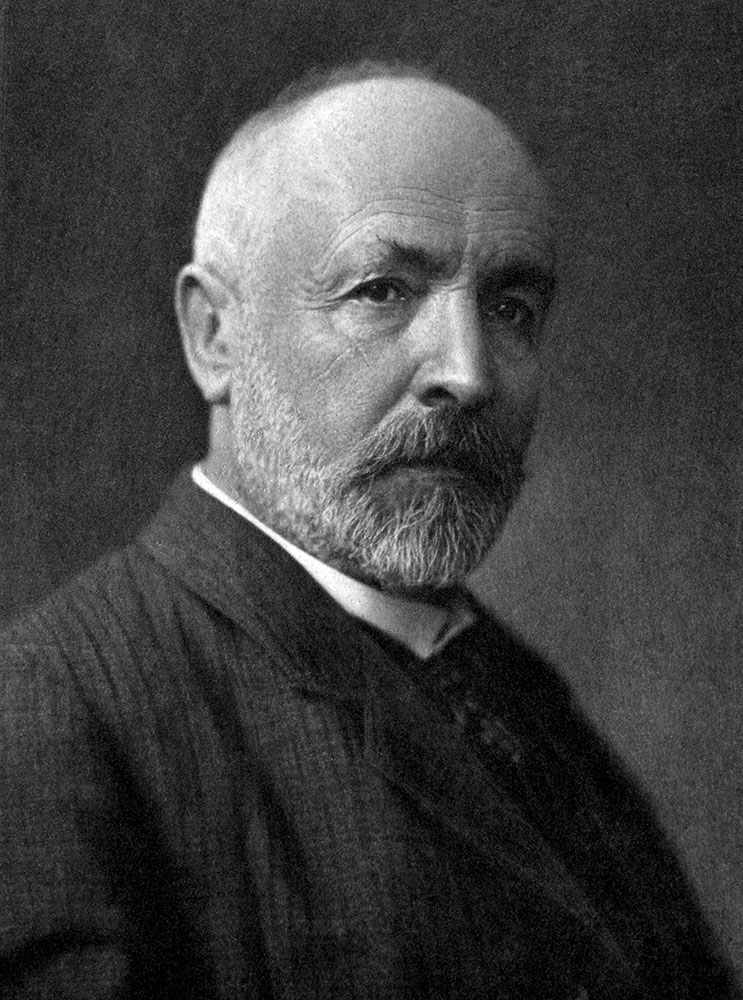
\includegraphics{img_073.jpg}
\caption[盖奥尔格·康托尔。]
  {盖奥尔格·康托尔}
\end{figure}

如果把这种方法用于对话中提出的“伟大数学家的完备名单”这个更具体的例子,这一差别就会变得更为清楚。对角线本身是“Dboups”。如果我们完成所要求的对角线减法,就能从中得到“Cantor”[康托尔]。这样就有两种可能的结论。如果你坚信这张表是完全的,那你必须下结论说康托尔不是伟大的数学家,因为他的名字和表中所有的名字均不同。另一方面,如果你坚信康托尔的确是个伟大的数学家,那你必须下结论说这张“伟大数学家的完备名单”是不完全的,因为康托尔的名字没有列在表上!(那些对两者都坚信的人将多么不幸!)前一种情况相应于我们的证明:“蓝对角”$[N]$不是原始递归的;后一种情况相应于康托尔的证明:实数表是不完全的。

康托尔的证明按字面上的意义使用了一条对角线。而其它的“对角线”证明则基于一个更加一般的观念,这个观念是从该词的几何意义中抽象出来的。对角线法的本质在于以两种不同的方式使用同一个整数——或者可以说在两个不同层次上使用同一个整数——多亏了这样人们才可能在某个预先给定的序列外面造出一个项来。这个整数一会儿被用作一个纵向索引,另一会儿被用作一个横向索引。这在康托尔的构造中表现得很清楚。至于说函数“蓝对角”$[N]$,它涉及到在两个不同层次上使用同一个整数——首先作为一个蓝程序索引编号,然后再作为一个输入参数。

\section{对角线论证阴险的重复}

初看起来,康托尔的论证似乎不足以完全使人信服。难道没有办法摆脱它吗?或许把从对角线上构造出来的数$d$扔进去,就可能得到一张完全的表。如果你在打这个主意,那你将看到把数$d$扔进去根本于事无补,因为一旦你为它在表中指定了一个位置,对这张新表又可以使用对角线法,能构造出一个不在这张新表中的数$d'$。无论你重复多少次下列操作:用对角线法构造一个数,然后把它扔进表中以形成一个“更完全”的表,你仍然无法逃出康托尔方法的巨掌。你甚至可以试着去构造一张实数表,以某种方式提防着康托尔对角线法的全套明枪暗箭以及它的阴险重复,设法战胜它。这是一个有趣的练习。但如果你动手试试看,就会发现无论你怎样腾挪躲闪,还是跑不出康托尔的手心。可以说任何自称构成了“包括全部实数的表”之举,都是搬石头砸自己的脚。

康托尔对角线法的可重复性有点像乌龟那种毒辣手法的可重复性。乌龟用这个办法一个接一个地破坏了螃蟹那些“保真度”越来越高——至少螃蟹希望如此——越来越“完备”的唱机。这个办法就是为每台唱机创作出一支特定的歌,使它不能用那台唱机来播放。康托尔的计谋和乌龟的计谋都具有这种奇妙的可重复性,这可不是巧合。事实上,《对位藏头诗》本来就应当被命名为《对角藏头诗》。正像乌龟微妙地暗示给天真的阿基里斯的那样,发生在《对位藏头诗》中的事件,正是哥德尔用来证明\emph{不完全性定理}的那个构造的一种形象化解释。由此可见,哥德尔的构造也很像一个对角线方法。这一点在下面两章中将变得很清楚。

\section{从BlooP到FlooP}

至此,我们已经用以BlooP语言写的程序为工具,定义了自然数上的原始递归函数和原始递归谓词所组成的类。我们也表明了BlooP不能囊括全部可用词语定义的自然数上的函数。我们甚至还用康托尔的对角线法构造了一个“非BlooP可编程的”函数,即“蓝对角”$[N]$。为什么在BlooP中不能表示“蓝对角”呢?是否能改进一下BlooP,以使得“蓝对角”成为可表示的呢?

BlooP的根本特征就是其中循环的有界性。如果我们抛掉对循环的这种要求,发明另一种语言,称其为FlooP(英文Free有“自由”的意思,我们借此表明FlooP的循环是自由的),会出现什么情况呢?FlooP除掉一点之外与BlooP完全相同:在FlooP中我们既可以用无顶的循环,也可以用有顶的循环(虽然在FlooP中写循环语句时注明其顶的唯一理由是为了好看)。这些新的循环将被称为\inst{MU-LOOP}($\mu$循环)。这是为了遵守数理逻辑中的约定:在其中“自由”搜索(无界搜索)通常被注上一个叫“$\mu$算子”的符号。因此,FlooP中的循环语句看上去会是这样的:
\begin{center}
\begin{tabular}{l@{\qquad}l}
\inst{MU-LOOP}: & $\mu$循环\\
\BEGINBLOCK{n}  &  第$n$块开始\\
\multicolumn1c{$\vdots$}\\
\ENDBLOCK{n};   & 第$n$块结束
\end{tabular}
\end{center}

这种特性使得我们可以用FlooP为“妙极性质”或“乌龟性质”这样的性质写测试程序——而这样的测试程序我们用BlooP是无法写出的,因为其中的搜索或许会无穷无尽。我将把对妙极性的测试程序留给有兴趣的读者自己去写,在这个测试中要实现下列功能:
\begin{enumerate}
\item 如果其输入$N$是妙极的,则程序结束,给出答案\inst{YES}。
\item 若$N$是非妙极的,但导致了一个不同于$1$-$4$-$2$-$1$-$4$-$2$-$1$\ldots\ 的封闭循环,则程序停止,给出答案\inst{NO}。
\item 若$N$是非妙极的,而且导致一个“无穷上升过程”,程序将不会结束。以这种方式,FlooP的不回答就是回答。FlooP的不回答就像赵州用“无”来“废问”一样。
\end{enumerate}
在第3种情况下,具有讽刺意味的是:输出变量\inst{OUTPUT}的值一直是\inst{NO},但我们又一直无法得到它,因为程序仍在不停地运转。这个讨厌的第三种可能性是我们写自由循环时所必须付出的代价。在所有包含了\inst{MU-LOOP}的FlooP程序中,无终止总是一种理论上的可能性。当然,有许多FlooP程序实际上相对于其所有可能的输入值都是能终止的。例如像我前面提到过的,大多数研究过妙极性的人都认为像上面提出的那样一个FlooP程序将总是能终止的,而且每次的答案都是\inst{YES}。

\section{有终止和无终止的FlooP程序}

一个看起来很吸引人的想法是:最好能把FlooP过程分成两类:“有终止过程”和“无终止过程”。一个“有终止过程”无论输入什么都将终止,尽管其中的循环具有“$\mu$性质”。而对一个“无终止过程”来说,则输入中至少有一种选择会使它永远运行下去。如果对每个FlooP程序,我们通过某种复杂的检验总能说出它属于哪一类,这将会有某种相当显著的效果(我们很快就会看到)。不必说,这种类别检测操作本身也必须是个有终止操作——否则就什么也得不到了!

\section{图灵的妙计}

我们立刻就会想到,可以让一个BlooP过程完成这个检验。但BlooP过程只接收数字输入,不能接收程序!不过,我们可以解决这问题……只要用数字对程序进行编码就行了!这个巧妙的计策只不过是哥德尔配数法的许多表现形式中的另一种罢了。令FlooP字母表中的五十六个字符分别对应于“密码子”$901$、$902$……$956$。这样每个FlooP程序就得到了一个相当长的哥德尔数。例如,那个最短的BlooP函数(它同时也是一个有终止的FlooP程序)——
\begin{center}
\begin{tabular}{l}
\PROCEDURE{A}{B} \\
\BEGINBLOCK{0}   \\
\ENDBLOCK{0}
\end{tabular}
\end{center}
——将得到一个哥德尔数,它的一部分如下所示:
\[
\setlength\arraycolsep{1pt}
\begin{array}{*{11}{c}}
904, & 905, & 906, & 909, & 914, & 905, & ........, &
905, & 914, & 904, & 955, \\
\inst{D} & \inst{E} & \inst{F} & \inst{I} & \inst{N} &
\inst{E} &  & \inst{E} & \inst{N} & \inst{D} &.
\end{array}
\]

现在我们的计划是写一个名为“\inst{TERMINATOR?}”的BlooP测试,其功能是:如果被其输入数字所编码的那个FlooP程序是有终止的,则回答\inst{YES},否则回答\inst{NO}。用这个办法就可以把这个任务交给机器去完成。如果走运,就能把有终止过程和无终止过程分开了。但是,阿兰·图灵给出的一个精巧的论证表明,任何BlooP程序都不能一贯正确地完成这种区分工作。图灵所用的技巧实际上和哥德尔的技巧基本相同,因此也密切联系于康托尔的对角线技巧。我们将不在这里把它给出来——只需说基本想法是往“终止检验程序”中送入它自己的哥德尔数。但情况并非如此简单,因为这很像设法在一个句子内部完整地引用它自己。你必须对引号也加引号,如此进行下去。这似乎会导致一个无穷回归。但是,图灵指出了一种技巧,可以把一个程序自身的哥德尔数送给它。对这同一个问题在另一个环境下的解决将在下一章中给出。本章里,我们将沿另一条途径来达到相同的目的,即证明不可能构成一个终止测试器。如果有些读者希望看到图灵方案的一个漂亮而又简单的表示,我推荐文献目录中提到的霍尔和艾利森[Hoare; Allison]的著作。

\section{终止测试器将是法力无边的}

在我们摧毁这个观念之前,让我们描述一下为什么说掌握了终止测试器将是一件值得大书特书的事:在某种意义上说,这就像有了一支法力无边的魔杖,用它可以轻而易举地解决数论中的一切问题。例如,假设我们想知道哥德巴赫变奏是否是个真实的猜想,也就是要问,是否所有自然数都具有乌龟性质?我们将首先写一个叫“\inst{TORTOISE?}”的FlooP测试,它检查它的输入是否具有乌龟性质。现在这个过程的缺点——即如果乌龟性质不成立,程序将不终止——反倒成了一个优点!因为现在我们可以把过程\inst{TORTOISE?}送入终止测试器。如果它回答\inst{YES},那意味着\inst{TORTOISE?}对一切输入值都将要终止——换句话说,所有自然数都有乌龟性质。如果它回答\inst{NO},那我们就知道存在一个具有阿基里斯性质的数。具有讽刺意义的是,我们根本没有实际使用\inst{TORTOISE?}程序——只是对它做了一次检查!

把数论中的每个问题编成程序,然后用一个终止测试器对它们来一个“一揽子解决”,这个主意有点像前面提过的那个测试公案的纯正性的想法:把公案编码在一个折叠的串中,然后去检查这个折叠的串是否具有佛性。正如阿基里斯所提示的那样,或许我们希望得到的信息在某一种表示法中比在另一种表示法中“更接近表面”。

\section{F库、索引编号和绿程序}

好,白日梦到此收场。我们怎么能证明终止测试器是不可能造出来的呢?我们关于其不可能性的论据联系于下述思路:设法对FlooP运用对角线论证,就像我们对BlooP所做的那样。我们将会看到两种情形还是有一些微妙而又关键的差别的。

像我们对BlooP所做的那样,设想包括全部FlooP程序的库。我们叫它“F库”,然后对它进行那三种过滤操作,这样最后我们将得到:

\begin{block}
一个包含所有这样的待调用FlooP程序的完整库:这些程序计算那些恰有一个输入参数的函数。
\end{block}

让我们称这些特殊的FlooP程序为“绿程序”(因为它们可能“一路绿灯”——永远畅行无阻)。

现在正像我们为所有蓝程序指定了索引编号一样,我们也能为绿程序指定索引编号,即把它们排列在一个目录表中,每一列包括具有一定长度的所有绿程序,按字典顺序排列。

到此为止,对FlooP的处理完全照搬了对BlooP的处理。现在让我们看看是否还能照搬下一步:对角线技巧。如果我们试图定义下列对角线函数会怎样呢?
\[
\text{“绿对角”}[N]=1+\text{绿程序}\{\#N\}[N]
\]

突然,我们碰上一块暗礁:“绿对角”$[N]$这个函数可能无法为所有输入值$N$都提供明确定义的输出值。原因很简单:我们没有从F库中剔除那些无终止程序,因此就无法保证我们能为$N$的所有值计算出“绿对角”$[N]$来。有时我们会进入永无休止的计算。因此对角线论证不能在这种情况下使用,因为它要求对角线上的函数为所有可能的输入算出输出值。

\section{终止测试器提供给我们红程序}

为了弥补这个漏洞,我们将不得不使用一个终止测试器,如果它真的存在的话。因此让我们有意识地引入这样一个可疑的假设:它真的存在,并且用它作为我们的第四个过滤器。我们逐个检查表中的绿程序,去掉那些无终止的,这样最后我们将得到:

\begin{block}
一个包含所有这样的待调用FlooP程序的完整库:这些程序计算那些恰有一个输入参数的函数,并且对所有的输入值都能终止。
\end{block}

让我们称这些特殊的FlooP程序为“红程序”(因为它们早晚会碰上个红灯——都必须停下来)。现在,对角线方法可以一显身手了。我们定义
\[
\text{“红对角”}[N]=1+\text{红程序}\{\#N\}[N]
\]
完全和对“蓝对角”的讨论平行,我们被迫断言“红对角”$[N]$是个良定义的单变量可计算函数,但不在红程序的目录表内,因此甚至在强有力的FlooP语言中也是不可计算的。或许现在该转到GlooP了?

\section{GlooP…}

是的,但GlooP是什么呢?如果说FlooP是去掉限制的BlooP,那么GlooP一定是去掉限制的FlooP。但一个限制怎么可能去掉两次呢?你怎么能构造一个比FlooP更强有力的语言呢?在“红对角”中,我们已经发现了一个函数,我们人知道如何去求它的值——求值方法已经明确地用自然语言描述出来了——但似乎不能用FlooP语言编出程序来完成这项工作。这是一个尖锐的二律背反,因为还没有人曾经发现过比FlooP更强有力的计算机语言。

有人曾经详尽地研究过计算机语言的能力,我们不必自己再去做这项工作,只须报告这样一项结果:有一大批计算机语言可以被证明是与FlooP具有完全相同的描述能力的,这就是说:任何一个可以用其中某种语言编程序完成的计算过程,必然能用所有这些语言中的任何一个来编程序完成。奇怪的是,几乎任何设计计算机语言的合理企图,都以构造出这个类中的一个成员而告终——也就是说,造出了一种能力等价于FlooP的语言。当然,通过某种努力也可以构造出一种比这一类语言要弱一些的合理并有趣的计算机语言。显然,BlooP就是弱语言的一个例子,但这是一种例外,而不是规律。关键在于存在许多很自然的方式可以用来发明算法语言,而不同的人,循着不同的途径,往往最终创造出等价的语言。它们只有形式上的差别,能力是一样的。

\section{…是个神话}

事实上,绝大多数人都相信不会再有描述计算的能力强于FlooP及其等价物的语言了。这个假说在30年代被两个人互相独立地表述出来:阿兰·图灵——关于他,后面还会进一步介绍——和阿朗佐·丘奇,二十世纪杰出的逻辑学家之一。他们的结果被称为“丘奇—图灵论题”。如果我们接受这个论题,我们就必须下结论说“GlooP”是个神话——在FlooP中已经没有限制可以取消,无法通过“解放”来增强它的能力,像我们对BlooP做过的那样。

这把我们置于一种尴尬的境地,即断言人可以为$N$的任意值计算“红对角”,但无法编出程序让计算机来完成这项任务。因为,如果这项任务可以得到完成,那它一定是用FlooP语言来完成的。而根据任务的构造方式,它又不可能用FlooP来完成。这个结论实在太奇特了,致使我们得非常仔细地研究它赖以建立的基础。而在这当中,你会想起来,就有我们那个不牢靠的假设,即存在一个可以区别有终止和无终止的FlooP程序的判定过程。这个判定过程的想法本来就有点可疑,因为我们已经看到它的存在将导致数论中的所有问题以一种统一的方式被解决。现在我们有了双重的理由相信任何终止测试都是一种神话——根本就无法把FlooP程序装到一台“甩干机”里,把有终止程序和无终止程序分离开来。

怀疑论者可能会坚持说这不像对此类终止测试的不存在性的一个严格证明。这种反对意见是合理的。但是,图灵的方案更为严格地论证了这一点:用一个和FlooP同类的语言,不可能写出计算机程序,来对所有FlooP程序进行终止测试。

\section{丘奇—图灵论题}

让我们简略地回顾一下丘奇—图灵论题。我们将在第十七章中相当详细地讨论它——以及它的变种,而现在只需要叙述它的几种形式,把关于其价值和意义的讨论推迟到后面去完成。这里是三种相互联系的叙述此论题的方式:
\begin{enumerate}
\item 人所能计算的也就是机器所能计算的。
\item 机器所能计算的也就是FlooP所能计算的。
\item 人所能计算的也就是FlooP所能计算的\lnote{(即一般递归或部分递归)}。
\end{enumerate}

\section{术语解释:一般递归和部分递归}

在本章中,我们对数论中的一些概念及其与可计算函数理论的联系进行了广泛的阐述。这是一个广阔而兴旺的领域,是计算机科学和现代数学的一个吸引人的混合体。我们在结束本章之前,还要介绍一下我们曾与之打过交道的一些观念所对应的标准术语。

前面已经提到过,“BlooP可计算”是“原始递归”的同义语。现在FlooP可计算函数可以被分成两类:\pnum{1}那些能用有终止FlooP程序计算的被称为“一般递归的”,\pnum{2}那些只能用无终止FlooP程序计算的被称为“部分递归的”(对谓词有类似的定义)。人们常常只说“递归”,其意思是“一般递归”。

\section{TNT的能力}

有趣的是,TNT是如此有力,以致于不仅能体现全部原始递归谓词,而且能体现全部一般递归谓词。我们将不证明这些事实,因为这对我们的目标来说是没有必要的。我们的目标是说明TNT是不完全的。如果TNT不能体现某些原始或一般递归谓词,那这样的不完全就太“没意思”了。——因此我们应该使它能做到这一点。然后,再说明它具有某种有趣的不完全性。
